\chapter{High-Performance Regimes}\label{ch:HighPerformance}

The development of magnetic-confinement fusion into an economical form of power generation is characterized by two seemingly contrary requirements: first, a high level of energy confinement is necessary to reach the desired level of self-heating of the plasma by fusion products, satisfying triple-product requirements (\cref{eq:tripleproduct}).  At the same time, particle transport must be sufficient to avoid the deleterious effects of accumulated helium ``fusion ash'' and other impurities on fusion performance -- particularly important in the case of the high-$Z$ impurities from the metal plasma-facing walls necessary for reactor-scale devices \cite{Loarte2007}.

A number of operating scenarios, collectively termed ``high confinement'' or H-modes\cite{Wagner1982,Keilhacker1984}, satisfying these requirements have been developed.  The ``low confinement'' or L-mode operating baseline of energy confinement is characterized through an extensive multi-machine scaling study \cite{Yushmanov1990} by the ITER-89 scaling,

\begin{equation}\label{eq:tau89}
 \tau_{E,ITER89} = 0.048 \times \overline{n}_e^{0.1} M^{0.5} I_p^{0.85} R^{1.2} a^{0.3} \kappa^{0.5} B_T^{0.2} P_{aux}^{-0.5}
\end{equation}

\noindent in which $\overline{n}_e$ is the line-averaged density ($\SI{e20}{\per\meter\cubed}$), $M$ is the atomic mass ($\si{amu}$), $I_p$ is the plasma current ($\si{\mega\ampere}$), $B_T$ is the toroidal field ($\si{T}$), $R$ and $a$ are the major and minor radii in $\si{\meter}$ (see \cref{fig:intro_geometry}), $\kappa$ is the elongation (see \cref{fig:intro_shaping}), and $P_{aux}$ is the externally-applied heating power ($\si{\mega\watt}$).  Compared to this baseline, H-modes represent a significant improvement in performance, with confinement -- here represented in a normalized sense by the $H$-factor, \ie

\begin{equation}\label{eq:H89}
 H_{89} = \frac{\tau_E}{\tau_{E,ITER89}}
\end{equation}

\noindent improved by roughly a factor of two compared to L-mode \cite{Greenwald1997}.

This improvement in confinement is due to the formation of a \emph{pedestal}, a transport barrier (see \cref{subsec:intro_barriers}) at the edge that greatly slows the transport of particles and/or energy out of the plasma, and accordingly forms a steep-gradient region in density and/or temperature at the edge.  Pedestal formation is achieved through strongly sheared flows in the plasma edge, driven in part by a radial electric field (the ``$E_r$ well'') and the resulting $\vec{E} \times \vec{B}$ flows in the pedestal.  While this flow is difficult to model due to the short scale lengths inherent to the pedestal \cite{Kagan2010,Landreman2012}, the role of edge $E_r$ and flows has been extensively studied both from an experimental \cite{Groebner1990,Burrell1999,Terry2000,McDermott2009a} and a theoretical \cite{Shaing1989,Biglari1990,Kim1991,Ware1996,Burrell1992} standpoint, as has the role of other edge fluctuations coupling into these flows in driving the transition into H-mode \cite{Schmitz2012}.  As the pedestal structure is known to set a strong constraint on the overall performance in high-confinement regimes \cite{Kinsey2011}, as well as determining the edge stability and heat exhaust properties of the regime, a firm understanding of the pedestal is essential for extrapolation of a high-performance regime to ITER and beyond.

This chapter provides an overview and comparison of different classes of established H-mode operation, particularly regarding their behaviors in the high energy confinement and low particle confinement required for a reactor.  Additionally, observations of Edge-Localized Modes (ELMs) \cite{Zohm1996} are addressed.  We then introduce the access conditions, operation, and global characteristics of \emph{I-mode} -- an alternate high-performance regime with a number of favorable characteristics for reactor operation, and the subject of the majprity of this thesis.

\begin{table*}[h]
 \pushtooutside
 \ttabbox{\caption{Typical operating parameters of tokamaks noted in this thesis, along with references to overviews of each machine.  \emph{Note:} all ITER values are projected.\note{check all values here}}\label{tab:tokamaks}}
 {\begin{tabular}{lcccccc}
  \toprule
  \emph{Device} &
  $R/a \;[\si{\meter}]$ &
  %$a \;[\si{\meter}]$ &
  $I_p\;[\si{\mega\ampere}]$ &
  $B_T \;[\si{\tesla}]$ &
  $\overline{n}_e \;[\SI{e19}{\per\meter\cubed}]$ &
  $T_{e0} \;[\si{\kilo\electronvolt}]$ &
%   heating &
  \emph{refs.}
  \\
  \midrule
  C-Mod (USA) &
  $\num{0.67/0.22}$ &
  %$\num{0.22}$ &
  $\le \num{2}$ &
  $3-8.1$ &
  $\le \num{50}$ &
  $\le \num{8}$ &
%   ICRF, LHRF &
  \cite{Hutchinson1994,Greenwald2007,Greenwald2013}
  \\
  DIII-D (USA) &
  $\num{1.67/0.67}$ &
  %$\num{0.67}$ &
  $1-3$ &
  $2.2$ &
  $\num{6}$ &
  $5-10$ &
%   ECRF, NBI &
  \cite{Luxon2002,Luxon2005a,Luxon2005}
  \\
  ASDEX-U (GER) &
  $\num{1.65/0.5}$ &
  %$\num{0.5}$ &
  $\sim 1$ &
  $3.9$ &
  $\num{7.5}$ &
  $2-3$ &
%   &
  \cite{Herrmann2003,Ryter2003,Stroth2013}
  \\
  JET (UK) &
  $\num{3.4/0.9}$ &
  $3-4$ &
  $3.8$ &
  $\num{5}$ &
  $10-20$ &
%   &
  \cite{McDonald2008,Romanelli2013}
  \\
  JT-60U (JAP) &
  $\num{3.4/0.9}$ &
  $3-4$ &
  $4.8$ &
  $\num{5}$ &
  $10-20$ &
%   &
  \cite{Kamada2002,Kitsunezaki2002}
  \\
  JFT-2M (JAP) &
  $\num{1.3/0.35}$ &
  $0.5$ &
  $2.2$ &
  $\num{5}$ &
  $1-2$ &
%   &
  \cite{Kusama2006,Miura2006}
  \\
  ITER* &
  $\num{6.2/2.0}$ &
  $15$ &
  $5.3$ &
  $\num{10}$ &
  $10$ &
%   &
  \cite{Shimada2007,ITER1999,Doyle2007}
  \\
  \bottomrule
 \end{tabular}}
\end{table*}

\section{ELM-Free H-Mode}\label{sec:hcr_elmfree}

\begin{figure}[t]
 \pushtooutside
 \fcapside[65mm]{\caption[Characteristic traces of transient ELM-free H-modes.]{Characteristic traces of transient ELM-free H-modes, highlighted on the traces (\cref{sec:hcr_elmfree}).  After the L-H transition, density and thermal pressure (and therefore fusion reaction rate and stored energy) rise, while turbulent particle transport is reduced, as seen by the drop in edge $D_\alpha$ light and suppression of turbulence.  However, radiated power rises due to impurity accumulation -- when radiated power reaches a level comparable to total heating power, the plasma drops back into L-mode.}\label{fig:hcr_elmfree}}{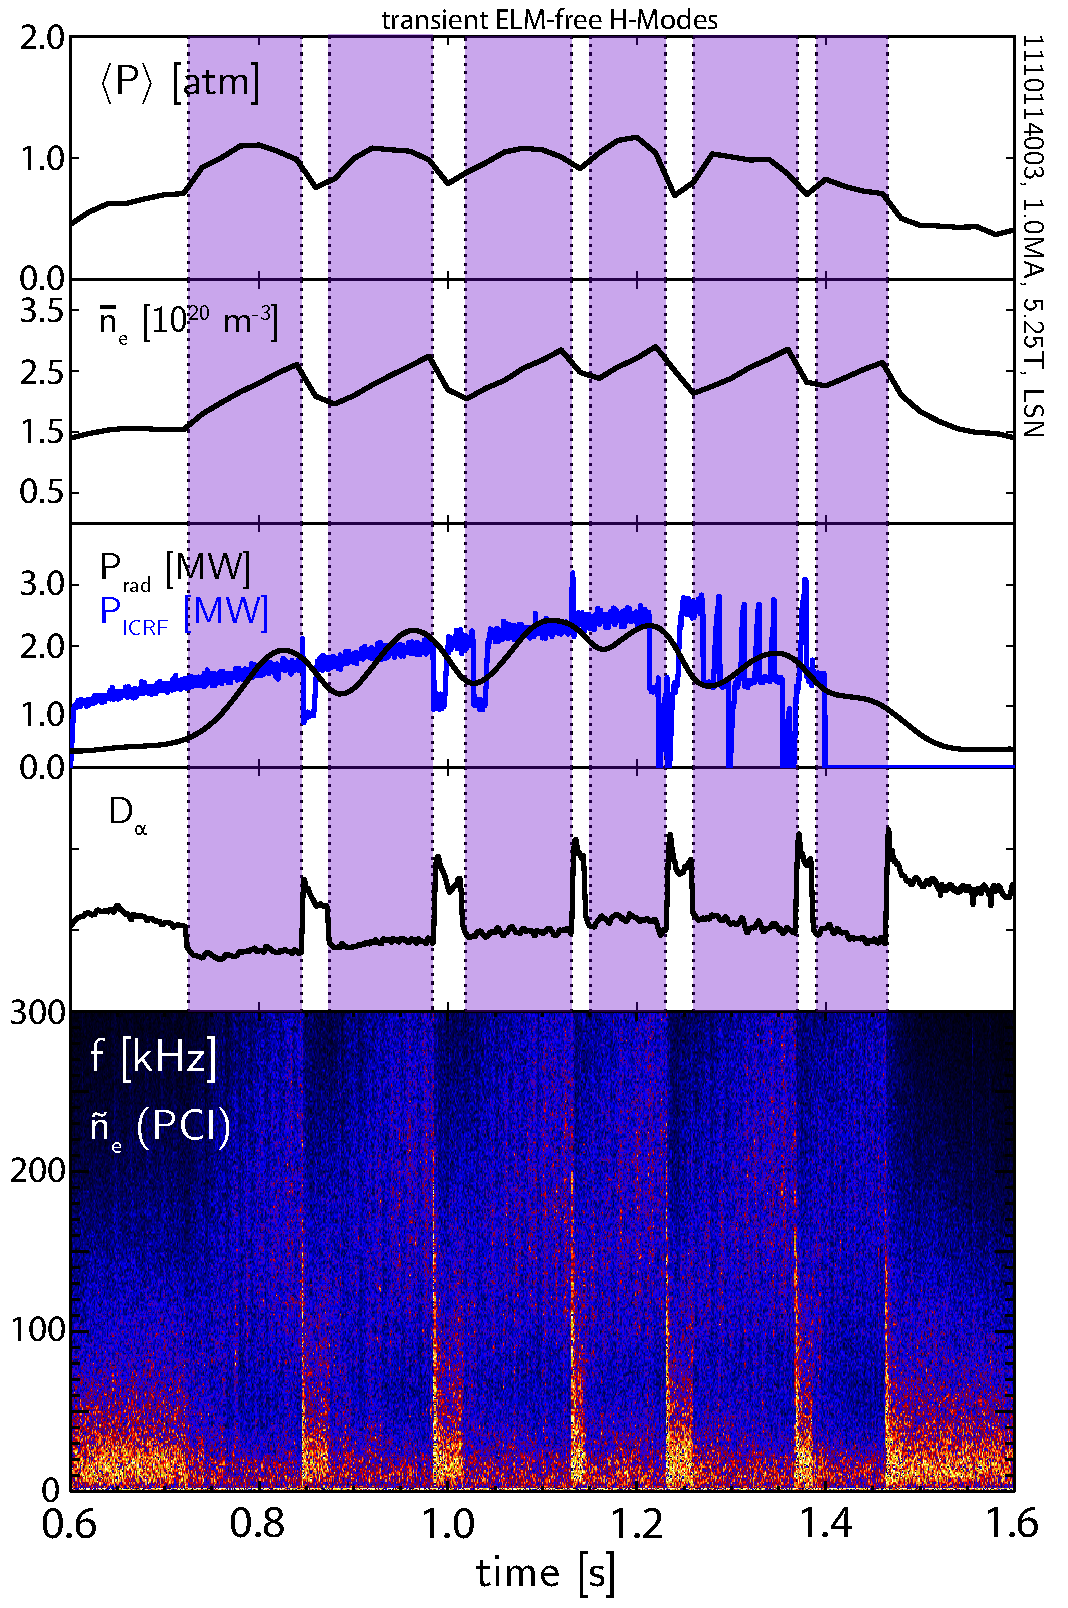
\includegraphics[width=100mm]{graphics/HighPerformanceRegimes/trace_1110114003.pdf}}
\end{figure}

At moderate levels of heating power above the L-H threshold \cite{Martin2008},

\begin{equation}\label{eq:Pthres}
 \begin{aligned}
  P_{thres} &= 0.0488 \times \overline{n}_e^{0.717} B_T^{0.803} S^{0.941} \quad [\si{\mega\watt}]\\
  S &= (2\pi)^2 aR \sqrt{\kappa}
 \end{aligned}
\end{equation}

\noindent ($\overline{n}_e$ is the line-averaged density in $\SI{e20}{\per\meter\cubed}$, $B_T$ in $\si{\tesla}$, and $S$ is the plasma surface area in $\si{\meter\squared}$) the plasma enters a transient \emph{ELM-free H-mode}, in which an H-mode forms without exhibiting large edge-localized modes (ELMs) \cite{Zohm1996,Suttrop2000a}.  ELM-free H-modes exhibit high levels of both energy and particle confinement ($H_{89} \sim 2$), resulting in strong density and temperature pedestals \cite{Hubbard2000,Hatae1998}.  The plasma stored energy, global pressure, and density rise monotonically after the L-H transition (shown in \cref{fig:hcr_elmfree}), as does the edge pressure gradient \cite{Breger1998}.  This, however, is unsustainable -- the increased particle confinement causes impurities to accumulate in the plasma, increasing the power lost to radiative effects.  Above $P_{rad}/P_{in} \sim 0.5$ confinement degrades due to cooling at the edge, and the H-mode terminates as the radiated power approaches the total 
heating power, an event termed the ``radiative collapse'' \cite{Greenwald1997}.

As a result, the conventional ELM-free H-mode is an inherently transient state for the plasma -- the excessive particle confinement and resulting radiative losses tend to drop the plasma back into L-mode, although under certain conditions the edge pressure gradient may grow sufficiently to instead transition into an ELMy H-mode \cite{Breger1998}.  This demonstrates the necessity of some form of density regulation in high-performance regimes to control and flush impurities from the plasma, allowing stationary operation.\nicesectionending

\section{ELMy H-Mode}\label{sec:hcr_elmy}

\subsection{ELMy H-Mode Operation}\label{subsec:hcr_elmy_ped}

\begin{figure}[p]
 \pushtooutside
 \fcapside[65mm]{\caption[Characteristic traces of a steady ELMy H-mode.]{Characteristic traces of a steady ELMy H-mode (\cref{sec:hcr_elmy}).  Density and radiated power rise after the L-H transition, but stabilize as the periodic relaxation of the pedestal regulates and flushes impurities from the plasma.  ELM bursts are visible as spikes on the edge $D_\alpha$ signal.}\label{fig:hcr_elmy}}{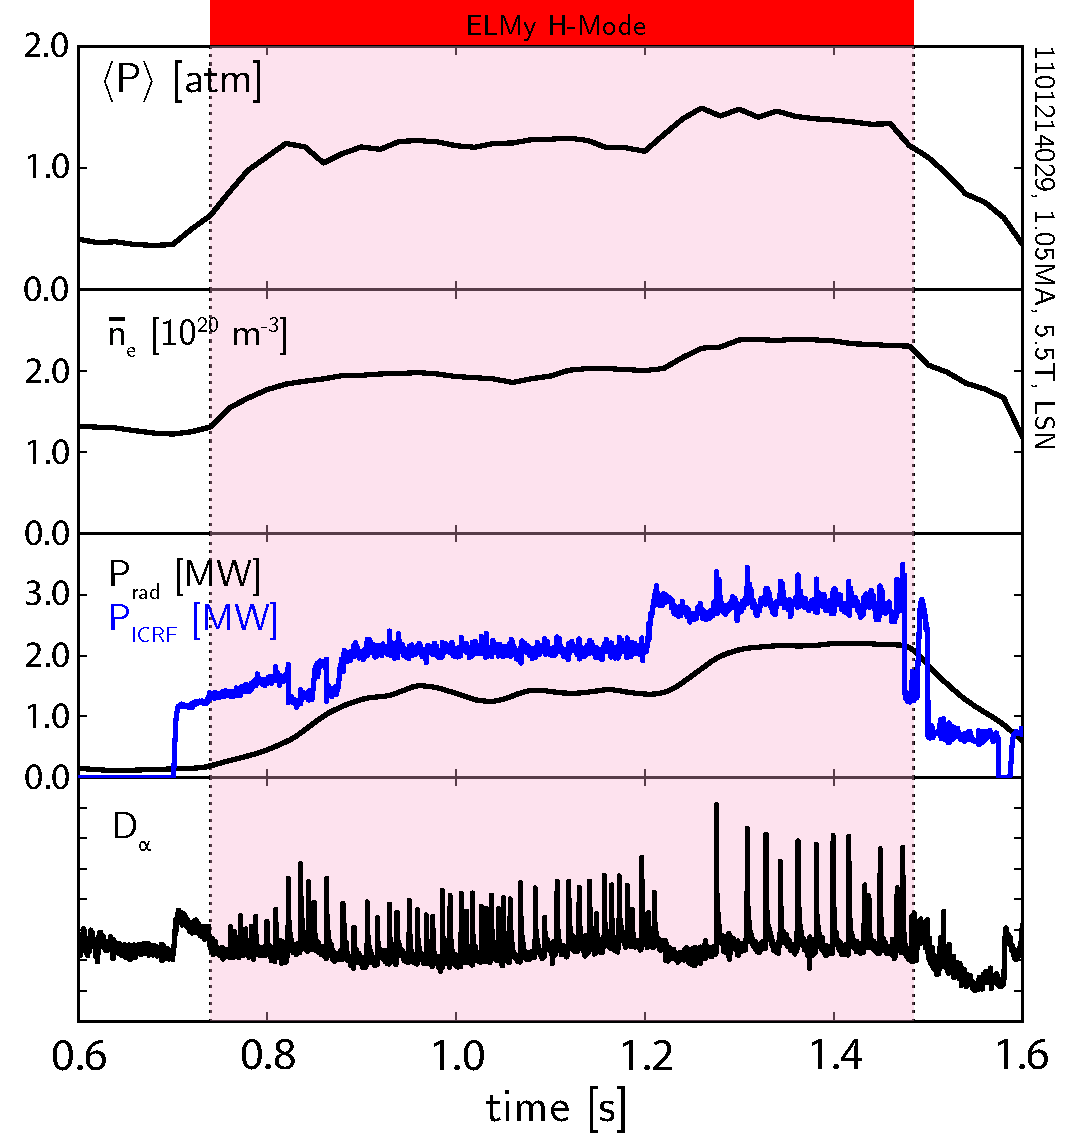
\includegraphics[width=100mm]{graphics/HighPerformanceRegimes/trace_1101214029.pdf}}
\end{figure}

\begin{figure}[p]
 \pushtooutside
 \fcapside[65mm]{\caption[ELMy H-mode pedestal density and temperature on a fixed-$\beta_{p,ped}$ line.]{ELMy H-mode pedestals from experiments on Alcator C-Mod and DIII-D, with matched dimensionless parameters between the two machines \note{elaborate on matching?}.  Pedestal densities and temperatures are shown normalized to poloidal field (which accounts for differences in plasma current) such that hyperbolae in the parameter space are curves of constant poloidal beta.  In the dimensionless match, ELMy H-mode pedestals are, to lowest order, constrained to a curve of fixed $\beta_{p,ped}$.}\label{fig:hcr_elmybetas}}{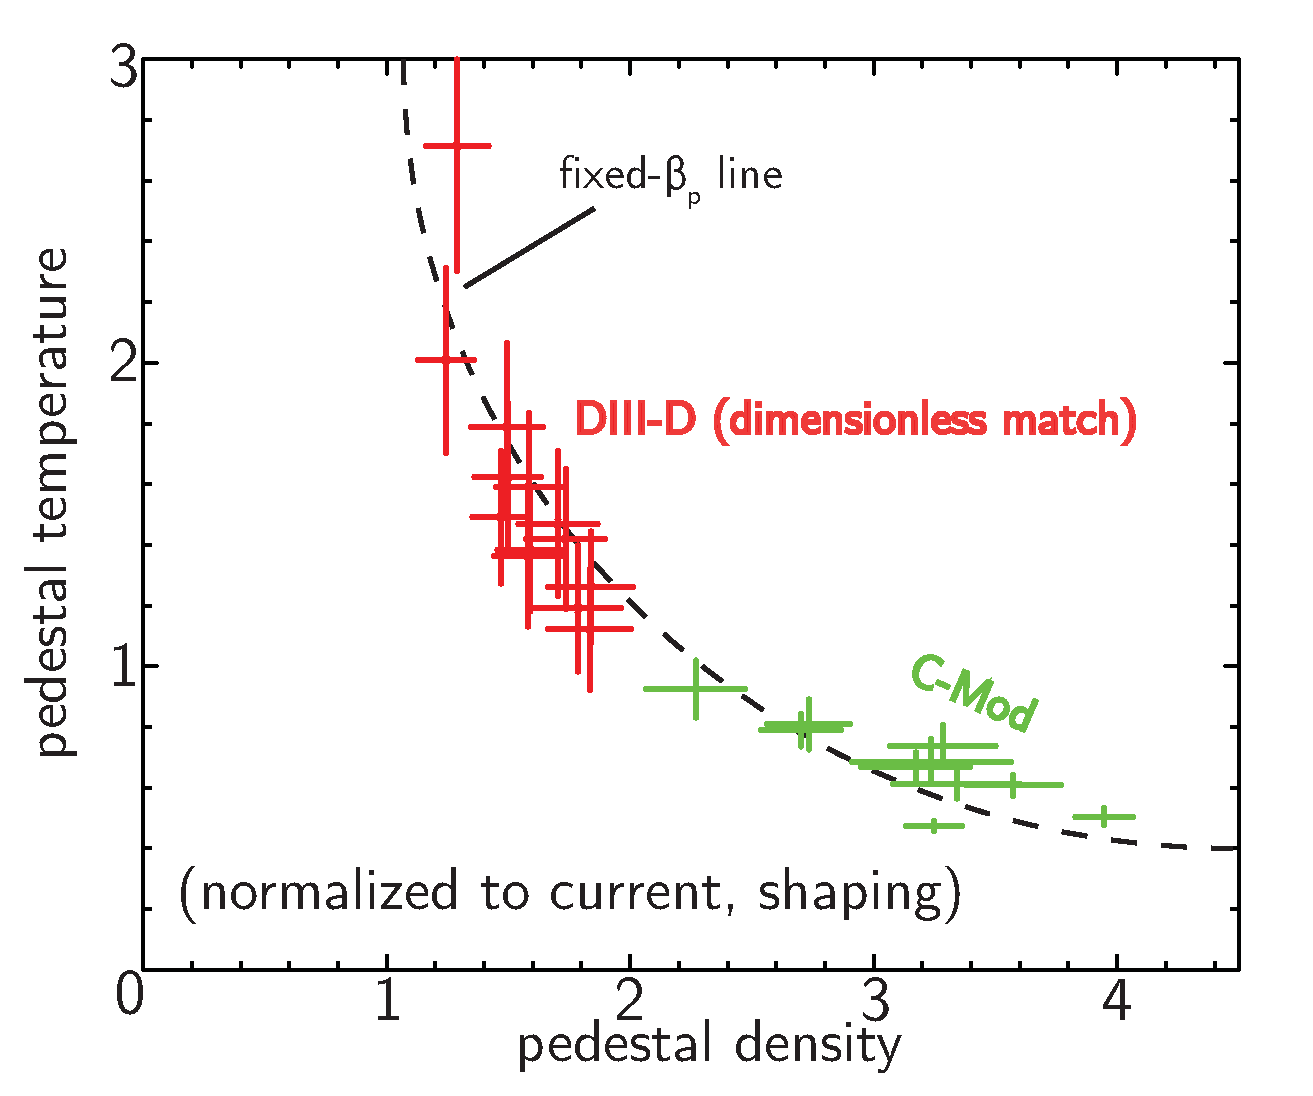
\includegraphics[width=100mm]{graphics/HighPerformanceRegimes/elmy_betas.pdf}}
\end{figure}

The first H-modes, observed in high-power experiments on ASDEX \cite{Wagner1982,Keilhacker1984}, exhibited a prompt decrease by roughly a factor of two in both particle and energy transport \cite{Wagner1982}.  The H-mode transition is marked by high edge temperatures and strong gradients -- the first H-modes were observed in divertor experiments on ASDEX, as the diverted configuration allows higher edge temperatures than are attainable in limited plasmas \cite{Keilhacker1984}.  Unlike ELM-free H-modes, however, the confinement is periodically degraded by \emph{Edge-Localized Modes} (ELMs), intermittent ``crashes'' in the pedestal expelling particles and energy into the SOL, with repetition rates ranging from a few ELM cycles per second to over $\SI{100}{\hertz}$, which drives sufficient particle transport to flush impurities from the plasma and allow stationary operation \cite{Keilhacker1984,Zohm1996}.  The ELMy H-mode forms a strong pedestal in both density and temperature, although at lower electron-ion coupling rates the ion pedestal may be wider \cite{Groebner1998a} -- due to profile stiffness in the core, this supports high temperatures and pressures and good global performance \cite{Greenwald1997,Suttrop2000,Schneider2013}.  Moreover, the ELMy H-mode is readily attainable on all major tokamak experiments, although ELMy H-modes on C-Mod require an atypical shape \cite{Hughes2012,Hughes2013}, as well as at a broad range of collisionalities and operating densities.  Here we define the collisionality (normalized collision frequency) by \cite{Sauter1999},

\begin{equation}\label{eq:nustar}
 \begin{aligned}
 \nu^* &= \frac{\nu_{eff}}{\nu_{bounce}} = \frac{qR\nu_{ei}}{\varepsilon^{3/2} v_{Th,e}}\\ &= \left(\num{6.921e-18}\right) \frac{Rqn_e Z_{eff} \ln \Lambda_e}{\varepsilon^{3/2} T_e^2}
 \end{aligned}
\end{equation}

\noindent with electron density $n_e$ in $\si{\per\meter\cubed}$ and temperature in $\si{\electronvolt}$, major radius $R$ in $\si{\meter}$, and with the Coulomb logarithm defined by $\ln \Lambda_e = 24 - \ln\left(\sqrt{n_e}/T_e\right)$.  Typically the pedestal collisionality is calculated by evaluating $n_e$, $T_e$, and $q$ at the 95\% flux surface.  The operating density range is expressed in terms of the Greenwald density limit \cite{Greenwald1988},

\begin{equation}\label{eq:GDL}
  n_{Gr} = \frac{I_p}{\pi a^2} \qquad f_{Gr} = \frac{\overline{n}_e}{n_{Gr}}
\end{equation}

\noindent with $I_p$ in $\si{\mega\ampere}$ and $a$ in $\si{\meter}$ yielding density in $\SI{e20}{\per\meter\cubed}$.  ELMy H-mode operation is possible with Greenwald fractions ranging from $f_{Gr} \sim 0.3-1.0$, although confinement degrades severely as $f_{Gr}$ approaches unity \cite{Saibene1999}.  As such, the ELMy H-mode is considered the baseline for ITER operation \cite{ITER1999,Shimada2007}.  Analysis of a multi-machine database \cite{Christiansen1992} led to the development of the ITER98y2 H-mode confinement scaling \cite{ITER1999}\gnote{check $P_{net}$ vs $P_{loss}$},

\begin{align}
 \tau_{ITER98y2} &= 0.0562 \times \overline{n}_e^{0.41} M^{0.19} I_p^{0.93} R^{1.39} a^{0.58} \kappa^{0.78} B_T^{0.15} P_{net}^{-0.69}\label{eq:tau98}\\
 H_{98} &= \frac{\tau_E}{\tau_{E,ITER98y2}}\label{eq:H98}
\end{align}

\noindent in which $\overline{n}_e$ is the line-averaged density ($\SI{e19}{\per\meter\cubed}$), $M$ is the atomic mass ($\si{amu}$), $I_p$ is the plasma current ($\si{\mega\ampere}$), $B_T$ is the toroidal field ($\si{T}$), $R$ and $a$ are the major and minor radii in $\si{\meter}$ (see \cref{fig:intro_geometry}), $\kappa$ is the elongation (see \cref{fig:intro_shaping}), and $P_{net}$ is the net heating power defined in \cref{eq:pnet} ($\si{\mega\watt}$).

Due to the importance of pedestal structure on overall performance \cite{Kinsey2011}, a number of models for the pedestal width and height in ELMy H-mode have been proposed.  The ELMy H-mode pedestal has been observed to be limited in pressure gradient \cite{Connor1998,Urano2003} -- as the pedestal width on a given machine typically varies only over a small range \cite{Maggi2010,Schneider2013}, this constitutes (to lowest order approximation) a limit on the attainable pedestal height.  Models based on gyroradius limits, and their expected effects on the growth rates of turbulent modes compared to the $\vec{E}\times\vec{B}$ shearing rate, have been proposed \cite{Groebner1998a,Beurskens2011}.  However, this has been discounted in favor of a model based on poloidal beta limits, $\beta_p = 2\mu_0 p/B_p^2$, both by experiments varying density and temperature at fixed $p_{ped}$ \cite{Osborne1998} and by isotope-mass-difference experiments \cite{Urano2008} (both of which vary the gyroradius without varying $\beta_{
p,ped}$).  These models are described in more detail in \cref{sec:mod_empirical}.

On smaller machines, ELMs provide sufficient impurity transport to allow stationary operation without seriously impacting energy confinement \cite{Rice1999}.  However, the transient power load from the ELM heat pulse is consistently observed to be $20-30\%$ of the input heating power \cite{Suttrop2003}, resulting in ELM energy losses reaching $2-6\%$ of the total stored energy -- on ITER, this results in heat pulses as high as $\SI{80}{\mega\joule}$ reaching the divertor plate \cite{Leonard1999,Suttrop2000}.  As wall materials are generally limited to ELM heat loads of $\sim \SI{10}{\mega\joule}$ per ELM \cite{Federici2003}, uncontrolled large ELM pulses can seriously exceed tolerances for ITER plasma-facing wall and divertor materials \cite{Loarte2003,Federici2003}.  Thus, avoiding or mitigating large, deleterious ELMs is essential for ITER operation.

\subsection{Edge-Localized Modes \& Pedestal Limits}\label{subsec:hcr_elmy_fluct}

Early phenomenological experiments on DIII-D and ASDEX \cite{Zohm1996,Connor1998,Suttrop2000} classified ELMs into three broad categories:

\begin{description}
 \item[Type-I] \hfill \\
 Large, discrete ELMs.  Repetition rate $f_{ELM}$ rises with increasing heating power.  The ELM crash is preceded by broadband electromagnetic and density fluctuations.  Type-I ELMy pedestals are modeled to be at or near the ballooning stability boundary (described below).
 \item[Type-II] \hfill \\
 Smaller and faster than type-I, often termed ``grassy ELMs.''  No discernable $f_{ELM}$ dependence on heating power.  Found in strongly shaped plasmas between the first and second-stable regions for ballooning MHD.
 \item[Type-III] \hfill \\
 Small ELMs, $f_{ELM}$ decreases with increasing heating power.  Exhibit a coherent magnetic precursor fluctuation before the ELM crash.  Found only below a threshold pedestal temperature.
\end{description}

Early investigation of the ELMy pedestal, particularly in large type-I ELMs, associated the pedestal limit with a ``ballooning'' MHD instability -- these MHD modes are driven unstable by strong pressure gradients in the edge, expressed in terms of the parameter $\alpha_{MHD}$ for a general toroidal equilibrium \cite{Miller1998},

\begin{equation}\label{eq:alphaMHD}
 \alpha_{MHD} = - \frac{2}{(2\pi)^2} \frac{\partial V}{\partial \psi} \sqrt{\frac{V}{2\pi^2 R}} \mu_0 \frac{dp}{d\psi}
\end{equation}

\noindent This reduces to a more intuitive form for a cylindrical plasma \cite{Connor1978},

\begin{equation}\label{eq:alphaMHD_cyl}
 \alpha_{MHD} = -\frac{2Rq^2}{B_T^2} \nabla p
\end{equation}

\noindent with the $q^2/B_T^2$ factor effectively expressing the scaling as $\alpha_{MHD} \sim \nabla p / B_p^2$.  Type-I ELMy H-mode pedestals are typically found to be near a critical value for $\alpha_{MHD}$ dependant on the plasma shape \cite{Osborne1998} -- stronger shaping is associated with slower ELM frequencies and greater stabilization of type-I ELMs, consistent with ballooning MHD \cite{Zohm1996,Saibene1999,Urano2003}.  Due to the restricted width range for the pedestal on a given machine \cite{Maggi2010,Schneider2013}, the $\alpha_{MHD}$ limit reduces, to good approximation, to a limit on $\beta_{p}$ at the pedestal top \cite{Saibene1999,Urano2003}.  For example, points at matched shaping, field and current across a DIII-D/C-Mod similarity experiment, shown in \cref{fig:hcr_elmybetas}, lie on a fixed $n_e T_e$ line.  The transition from type-I to type-III ELMs with increasing density and decreasing temperature \cite{Saibene1999}, or alternately the transition from type-III ELMs just above the L-H transition to type-I ELMs with increasing heating power \cite{Connor1998}, is consistent with the transition from a resistive mode for type-III ELMs to the ideal MHD modes identified with type-I ELMs.

A naive ballooning MHD analysis, however, does not accurately capture the ELMy H-mode pedestal -- parallel observations of MHD stability in early ELMy H-modes also identified current-driven kink/peeling modes as a potential limiting instability, particularly at low collisionality \cite{Connor1998,Suttrop2000,Groebner1998a}.  This is particularly true in light of the \emph{bootstrap current}, an effect by which gradients in the plasma self-generate an electric current, given by \cite{Sauter1999}

\begin{equation}\label{eq:jboot}
 j_{boot} = I(\psi) p_e(\psi) \left[ \alpha \frac{dn_e}{d\psi} + \beta \frac{dT_e}{d\psi} + \gamma \frac{dT_i}{d\psi}\right]
\end{equation}

\noindent where $I(\psi) = RB_\phi$ is a flux function encoding the field, $p_e(\psi)$ is the electron pressure, and $\alpha$, $\beta$, and $\gamma$ are coefficients determined by the collisionality and trapped-particle fraction, ordered $\alpha > \beta > \gamma$.  Due to the strong density and temperature gradients in the pedestal, the local current density may be large enough for current-driven kink/peeling modes to be a concern.  

MHD models built on coupled peeling and ballooning MHD modes, as well as diamagnetic effects stabilizing ballooning modes with high toroidal mode number $n$ \cite{Suttrop2000}, have been developed \cite{Snyder2002,Turnbull2003} and successfully capture the MHD limits of the ELMy H-mode.  Moreover, turbulence studies based on the kinetic ballooning mode \cite{Tang1980} predict that the mode will limit the pressure gradient and width such that the pedestal width scales with $\beta_{p,ped}$ in a manner consistent with experimental observations, $\Delta_{ped} \sim \beta_{p,ped}^{1/2}$ \cite{Snyder2001}.  Turbulent fluctuations with an onset soon after the inter-ELM pressure pedestal gradient saturation have been observed \cite{Diallo2014}, but a definitive analysis is still ongoing.  A self-consistent model including both the MHD and turbulent constraints, EPED \cite{Snyder2009}, has been implemented and tested in multi-machine analyses \cite{Groebner2013}, including on DIII-D \cite{Snyder2012}, C-Mod \cite{Walk2012}, and KSTAR \cite{Han2013}.  The constraints of this model are discussed in detail in \cref{ch:Modeling}.

\subsection{Active ELM Control}\label{subsec:hcr_elmy_control}

In lights of the potential deleterious effects of large ELMs on ITER-scale devices \cite{Loarte2003,Federici2003}, mitigating or preventing large type-I ELMs in H-mode is of prime concern.  One engineering solution for active ELM control is the application of a \emph{resonant magnetic perturbation} (RMP) \cite{Evans2004,Moyer2005,Evans2006}.  This perturbation drives additional particle and energy losses along stochastic field lines crossing the edge, limiting the pedestal before a large ELM boundary is reached \cite{Evans2004,Moyer2005}.  Small perturbations (less than $1/1000$ the magnitude of the background magnetic field), for example that driven by an $n=3$ coil set on DIII-D \cite{Evans2004} or a variable $n=3,4,6$ set on MAST \cite{Kirk2013}, couples to the intrinsic error field caused by the toroidal-field coils to provide the resonant perturbation \cite{Moyer2005}.  Due to its resonant nature, the RMP effect is strongly sensitive on edge safety factor $q$, limiting the potential profiles possible for RMP ELM suppression \cite{Moyer2005}.  This results in a strong density pumpout, along with moderate decreases in pedestal temperature gradients, which relaxes the pedestal and maintains it in the peeling-ballooning stable region \cite{Evans2006,Snyder2012}.

Rather than attempting to eliminate the ELM instability, it is also possible to ``smooth out'' the ELM heat pulse using pellet pacing \cite{Baylor2013}.  Generally, the transient ELM power $P_{ELM} \sim f_{ELM} \Delta W_{ELM}$ is roughly fixed - thus smaller, faster ELMs expel the less energy per ELM for the same average power.  By triggering smaller, faster ELMs the heat load can be smoothed to a level closer to steady-state heat loads tolerable to divertor materials, rather than large transient heat pulses.  In pellet pacing, the sharp density increase locally introduced in the pedestal by the pellet triggers a high-$n$ ballooning mode, resulting in a small ELM.  In ITER-match experiments on DIII-D \cite{Baylor2013}, cryogenic Deuterium pellets fired at twelve times the expected ELM frequency (roughly $\SI{5}{\hertz}$) reduced the per-ELM energy loss from $8\%$ of total stored energy, $\SI{55}{\kilo\joule}$, to less than $0.5\%$ ($\SI{3}{\kilo\joule}$).  However, the question of feasibility of pellet pacing for ITER, as well as the potential for non-axisymmetric heat loading in the divertor due to the localized nature of the pellet perturbation, remain open for the applicability of the concept to ITER.

\subsection{Prospects for ELMy H-Mode}\label{subsec:hcr_elmy_prospects}

Though ELMy H-mode represents the most readily attainable high-performance regime, its applicability to ITER-scale devices hinges on the limitation, mitigation, or elimination of large ELMs and the associated heat loads on wall and divertor surfaces.  ELM losses from type-I ELMs tend to be smaller for a given $\beta_{p,ped}$ at higher density and lowe temperature, ultimately transitioning to type-III ELMs \cite{Urano2003}, however these plasmas tend to exhibit lower global confinement \cite{Saibene1999}.  Type-II ELMs may provide the necessary near-continuous heat exhaust, but access to the regime is narrow and highly sensitive to shaping \cite{Suttrop2003}.  Alternately, ELM heat loading in type-I regimes may be controlled or suppressed via engineering solutions (\ie RMP or pellet pacing) -- but these are similarly limited in availability, and are of uncertain extrapolation to ITER-scale devices.  Thus, recent efforts have also placed great emphasis on high-performance regimes that are naturally free of 
large ELMs.\nicesectionending

\section{ELM-Suppressed H-Modes}\label{sec:hcr_elmsuppressed}

In addition to H-modes exhibiting ELMs, classes of H-mode have been established capable of stationary operation with acceptable levels of particle transport (avoiding the radiative collapse and subsequent transient nature found in classical ELM-free H-modes) without exhibiting the bursty heat and particle transport driven by ELMs.  Rather, the pedestal is regulated by a continuous fluctuation localized in the pedestal.  Due to this attractive property, these regimes have been extensively researched\gnote{reword}.  The characteristics of two major types, the Quiescent H-mode (QH-mode) and Enhanced $D_\alpha$ (EDA) H-mode are presented here.

\subsection{QH-Mode}\label{subsec:hcr_qh}

The \emph{Quiescent H-mode} (QH-mode) was first observed on DIII-D \cite{Burrell2002,Groebner2001}, and subsequently achieved on ASDEX Upgrade \cite{Suttrop2003a}, JT-60U \cite{Sakamoto2004}, and JET \cite{Suttrop2005}.  In QH-mode operation, following a brief ELM-free or ELMing phase after the L-H transition, the plasma enters a state with steady averaged density and radiated power, indicating a lack of serious impurity accumulation, despite lacking ELM transport (evident from divertor $D_\alpha$ light, which is ``quiescent'' compared to the characteristic spikes driven by ELMs).  Although QH-mode requires lower densities (average density reduced by roughly a factor of two from comparable ELMy H-modes) with cryopumping for density control, access is otherwise robust, with successful operation across a broad range of shaping, safety factor, current and field \cite{Burrell2002}.  The regime is capable of stationary operation, with the mode sustained for most of the current flat-top on DIII-D ($\sim 25 \tau_E$) with very good confinement -- in cases with an internal transport barrier in addition to the pedestal (termed the ``Quiescent Double Barrier'' or QDB regime \cite{Burrell2001,Doyle2001,Greenfield2002}) a confinement metric of $\beta_N H_{89} \sim 7$ was reached (albeit for a briefer period, $\sim 5 \tau_E$), compared to $\beta_N H_{89} \sim 4$ found in ELMy H-modes on DIII-D \cite{Doyle2001}.  Here we use the normalized pressure metric \cite{Troyon1984}

\begin{equation}\label{eq:betan}
 \beta_N = \beta \frac{aB_T}{I_p}
\end{equation}

\noindent in $\si{\meter.\tesla\per\mega\ampere}$.  Similarly competitive confinement between QH-mode and ELMy H-mode is seen on ASDEX Upgrade and JET, although the mode on JT-60U is out-performed by ELMy H-mode \cite{Oyama2006}.  The pedestal density is reduced (comparable to the reduction in globally-averaged density) in QH-mode compared to ELMy H-mode, and excess fueling to the edge by gas puffing, pellet fueling, or wall outgassing destroys the QH-mode.  However, pedestal temperatures are typically somewhat higher \cite{Doyle2001}, thus the mode is found at ITER-relevant low collisionalities.  Pedestal pressure gradients are comparable to those found in ELMy H-mode, implying stabilization of the peeling-ballooning MHD modes typically associated with the ELM trigger \cite{Burrell2002}.\gnote{elaborate?}  A particularly strong $E_r$ well ($2-3$ times deeper than in comparable ELMy H-modes) is also observed in the QH-mode pedestal \cite{Greenfield2002}.

In place of bursty ELM transport, the pedestal in QH-mode is continuously regulated by the \emph{Edge Harmonic Oscillation} (EHO), an MHD mode observed in density, temperature, and magnetic fluctuations \cite{Burrell2002}.  The EHO is made up of distinct harmonics with toroidal mode numbers $n \sim 1-10$; these harmonics are directly observed in the particle flux at the divertor, indicating that the EHO is responsible for density regulation in QH-mode \cite{Doyle2001}.  MHD modeling approaches similar to that described in \cref{ch:Modeling} indicate that the EHO is a saturated peeling mode \cite{Snyder2007,Osborne2008,Snyder2012}.  This is consistent with the low pedestal collisionality in the QH-mode pedestal (lower collisionalities and higher bootstrap currents tends to drive the pedestal towards the peeling side of the peeling-ballooning MHD boundary, as described in \cref{ch:Modeling}), and with the observed localization of the EHO in the region of strongest $E_r$ and rotation shear \cite{Burrell2001}.  The saturated mode is driven by the strong rotation shear in the edge -- while this typically destabilizes low-$n$ MHD modes\gnote{pull ref 9 from Burrell2009?}, in the case of the EHO the magnetic component of the mode couples to the vacuum-vessel wall as the rotation spins up, providing the drag force necessary to saturate the mode at finite amplitude \cite{Burrell2009}.  This maintains the pedestal below the current-driven peeling boundary associated with the ELM trigger, providing the ELM suppression in QH-mode \cite{Snyder2012}.

Historically, QH-mode operation has required significant neutral-beam inputs directed counter the plasma current direction, providing the necessary rotation \cite{Burrell2002}.  However, counter-current beam operation drives significant fast-ion losses into the outer wall, necessitating operation with a large outer gap to avoid wall outgassing.  More recent experiments have successfully generated QH-modes with co-current beam injection \cite{Burrell2009} and with torque from non-axisymmetric magnetic fields \cite{Garofalo2011,Burrell2013}.  The latter is of particular importance, as it is not expected that the NBI systems on ITER will drive sufficient torque to produce QH-mode \cite{Garofalo2011}.  In addition to the requirement for externally-supplied torque to maintain the mode, QH-mode suffers from accumulation of high-$Z$ impurities -- while lower-$Z$ ions are flushed from the plasma by the EHO, high-$Z$ impurities tend to accumulate in the core \cite{Doyle2001,Suttrop2005}, which may present difficulties attaining QH-mode on metal-walled machines where high-$Z$ impurities dominate.  Nevertheless QH-mode is an attractive option for a reactor regime.

\subsection{EDA H-Mode}\label{subsec:hcr_eda}

\begin{figure}[t]
 \pushtooutside
 \fcapside[65mm]{\caption[Characteristic traces of an EDA H-mode on C-Mod.]{Characteristic traces of an EDA H-mode on C-Mod (\cref{subsec:hcr_eda}).  Following a brief ELM-free phase, the plasma density and radiated power stabilizes at a sustainable level.  The edge transport barrier is regulated by the continuous QCM fluctuation rather than bursty ELM transport.}\label{fig:hcr_eda}}{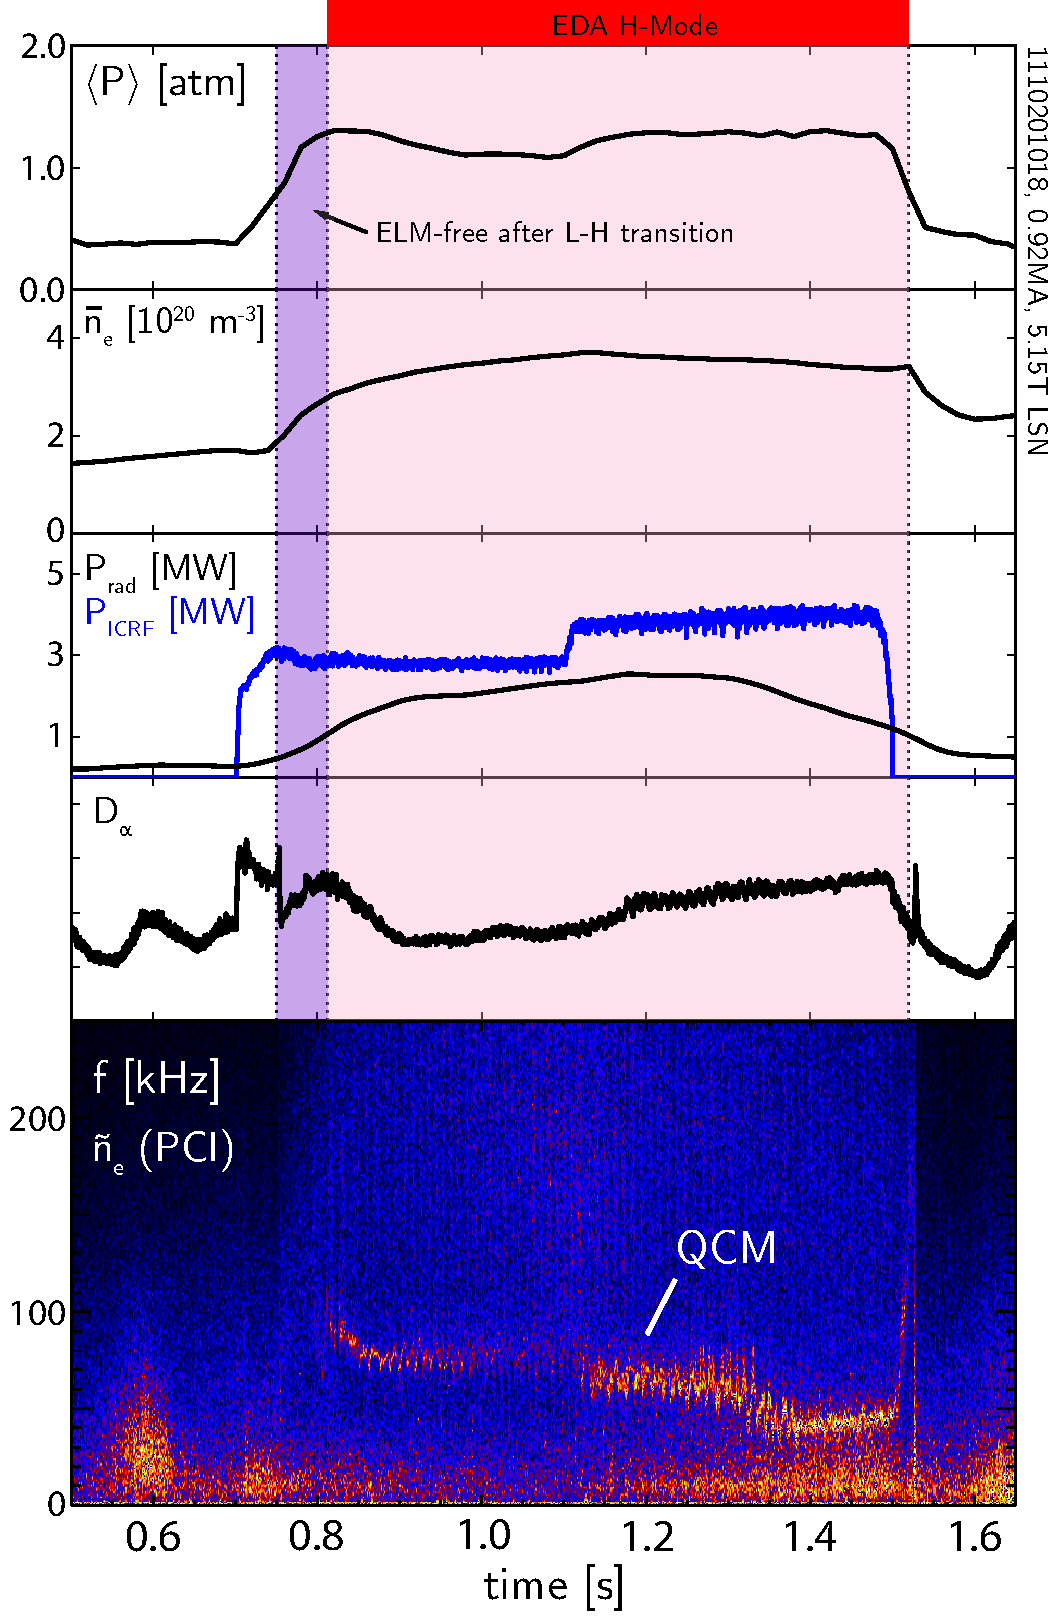
\includegraphics[width=100mm]{graphics/HighPerformanceRegimes/trace_1110201018.pdf}}
\end{figure}

The \emph{Enhanced $D_\alpha$ H-mode} (EDA H-mode) is a high-performance regime explored on the Alcator C-Mod tokamak \cite{Greenwald1999,Hubbard2001,Hughes2005}\gnote{time trace, fluctuations, profile comparison between EDA, ELMy}.  Along with transient ELM-free H-modes, the EDA regime is the customary approach to H-mode operation on C-Mod, unlike other major tokamak experiments; the Type-I ELMy H-mode typical on other devices requires an abnormal shaping to more easily reach the stability boundary associated with the ELM trigger on C-Mod \cite{Hughes2013}\gnote{make sure to elaborate on this in ELMy section or reference later}.  In EDA operation, the L-H transition is followed by a rise in radiated power and density similar to an ELM-free H-mode.  However, shortly thereafter the H-mode stabilizes at steady density \cite{Greenwald1999}, with the radiated power held at $P_{rad}/P_{in} \sim 30\%$ \cite{Hubbard1998}, allowing steady operation (maintained for most of the steady current phase, $\sim 10\tau_E$) and good performance, with $H_{89} \sim 1.9$, $H_{98} \sim 1$ \cite{Hubbard2001}.  Notably, modeling of the pedestal in EDA H-mode indicates energy confinement with potentially weaker degradation of $\tau_E$ with input heating power \cite{Hughes2002,Hughes2005,Hughes2006}\gnote{move this elsewhere?}.  Rather than bursty ELM transport, the EDA pedestal is regulated by a continuous density pumpout, with divertor $D_\alpha$ signals (indicative of the density exhaust from the plasma) recovering to near L-mode levels after an initial drop at the L-H transition\gnote{check this, reword?}.  Access to EDA H-mode is fairly robust, although it is strongly favored by higher collisionality ($\nu^* > 1$) and edge safety factor \cite{Hughes2002,Mossessian2002} and by strong shaping \cite{Mossessian2002}\gnote{define $\nu^*$ here, or earlier?}.  Although a higher collisionality is observed to be required at lower values of $q_{95}$, a collisionality threshold alone is insufficient to explain EDA access \cite{Hughes2002}.  Instead, EDA and ELM-free H-modes are separated in a phase space of collisionality and normalized pressure gradient ($\nu^*$-$\alpha_{MHD}$)\gnote{define $\alpha_{MHD}$ before here} -- however, the transition between the two regimes is soft, with the EDA smoothly appearing at higher pressure gradients and collisionalities rather than exhibiting a sharp transition \cite{Hughes2007a}.

While the pedestal pressure in EDA H-mode is comparable to that in ELMy H-mode, the pedestal profiles in EDA tend towards higher density and lower temperature -- this strongly alters the collisionality (consistent with the observed requirements for $\nu^* > 1$ for EDA access) and bootstrap current near the edge, with significant impact on MHD behavior.  The pedestal appears to be limited by transport effects rather than stability -- the pedestal is modeled to be stable to ideal MHD effects \cite{Mossessian2002,Hughes2013}, despite exhibiting a $\nabla p \sim I_p^2$ trend expected from a ballooning instability \cite{Hughes2006}\gnote{elaborate here, or elsewhere?}.  Instead, the pedestal density is determined by the interplay between an inward particle pinch and outward density transport.  Outward particle transport is decreases at higher currents (and therefore higher densities at fixed Greenwald fraction\gnote{explain or reword}), while the high pedestal density results in strong ionization in the scrape-off layer and an edge that is relatively opaque to neutrals \cite{Hubbard2007,Greenwald2007}.  As a result, the density will rise until the transport saturates -- additional fueling through the edge triggers minimal response, while a density drop is countered by increased particle particle confinement to recover the density, resulting in pedestal and global density values set by the plasma current, with weak dependence on other engineering parameters \cite{Hughes2007}.

The regulation of the pedestal in EDA H-mode is provided by the \emph{Quasi-Coherent Mode} (QCM), a field-aligned electromagnetic fluctuation localized in the steep-gradient region of the pedestal \cite{Hubbard2001,Terry2005,Mossessian2003}.  The QCM is a fairly narrow-band ($\delta f/f \sim 10\%$) mode strongly visible in density and magnetic fluctuations, with a centroid frequency of $50-200\;\si{\kilo\hertz}$ and a fairly short poloidal wavelength, $k_\theta \sim \SI{1.5}{\per\centi\meter}$ \cite{Terry2005}.  QCM fluctuations are visible in the density flux to the divertor, indicating that the QCM fluctuation is directly responsible for the particle transport through the EDA H-mode pedestal \cite{Greenwald2007,Terry2005}.  Numerical modeling of the EDA H-mode pedestal suggests a resistive ballooning mode (the collisional analogue to the ideal ballooning MHD mode found in ELMy H-modes\gnote{describe this in ELMy section}) for the QCM \cite{Mazurenko2002,Hughes2007a}.  This is consistent with experimental observations of the EDA pedestal -- the requirement of high collisionality (the QCM dissappears below $\nu^* \sim 0.1$) suggests a resistive effect \cite{Hughes2013}, while the favored high edge pressure gradient ($\alpha_{MHD}$) suggests a ballooning instability.  At high power and high edge pressure gradient, the QCM is replaced by small, high-frequency ELMs \cite{Mossessian2002,Mossessian2003,Hughes2007a}, potentially indicating that the pedestal is ``burning through'' the resistive-ballooning regulation of the pedestal and reaching the ideal MHD boundary associated with the ELM trigger.\gnote{ref here about high collisionality in other small-ELM regimes?}

The EDA H-mode presents another potential route to reactor-scale operation with naturally-suppressed large ELMs.  The regime is robustly accessible on C-Mod using only RF heating with no external momentum sources or non-axisymmetric magnetic coils, with good confinement and acceptable levels of impurity accumulation and radiated power consistent with high performance \cite{Hughes2011}.  Moreover, there is an extensive body of research studying the EDA H-mode on a machine with all-metal walls, with ITER-relevant heat flux and edge neutral behavior \cite{Hubbard2007,Greenwald2007}, and with similar electron-ion equilibration to that expected for ITER \cite{McDermott2009a}.  However, the necessary collisionality ($\nu^* > 1$) for the QCM fluctuation is significantly higher than the expected levels for the ITER pedestal ($\nu^* < 0.1$), inconsistent with unaided access to the EDA regime\gnote{where to go with this, mention shoelace?}.\nicesectionending

\section{I-Mode}\label{sec:hcr_imode}

In order for an H-mode regime to achieve stationary operation, there must be some form of relaxation of the density transport barrier -- either by intermittent bursts of transport due to ELMs, or through a continuous fluctuation regulating the particle confinement (as in the EDA and QH-modes).  However, each of these modes faces some level of increased particle confinement, as well as difficulties inherent in their operation -- the large type-I ELMs found in the most readily accessible ELMy H-mode on most tokamaks is incompatible with reactor-scale operation due to the large pulsed heat loads on wall and divertor materials \cite{Federici2003,Loarte2003}, while alternate H-modes are more restricted in their accessibility\gnote{reword this, shorter}.  Recent work on Alcator C-Mod has demonstrated a novel high-confinement regime, termed the \emph{I-mode}, which is unique in that it appears to completely decouple energy and particle transport, forming an H-mode-like temperature pedestal with the accompanying improvement in energy confinement, while maintaining an L-mode density profile and particle transport level.  I-mode exhibits several highly attractive properties for a reactor regime:

\begin{enumerate}
 \item The lack of a particle transport barrier or density pedestal maintains the desired level of impurity flushing from the plasma, avoiding excessive radiative losses
 \item I-mode appears to be generally stable against large ELMs, avoiding the excessive pulsed heat loads found in ELMs (of critical importance for ITER-scale devices) without externally-applied engineering controls
 \item appears to exhibit much weaker degradation of confinement with icreased heating power
\end{enumerate}

\noindent A firm understanding of the structure and stability of the I-mode pedestal is essential for the extrapolation of I-mode operation to larger devices, and will form the balance of this thesis.

\subsection{Access and Operation}\label{subsec:hcr_imode_access}

It has been long established that the orientation of the X-point (described in \cref{subsec:intro_toroidal}) relative to the vertical particle drifts (particularly the $\nabla B$ drift, \cref{eq:gradbdrift}) in the plasma column has a strong effect on plasma behavior, particularly flows in the edge \cite{LaBombard2004,Fenzi2005,Hubbard2007,LaBombard2008}.  Notably, in cases where the ion $\nabla B$ drift is directed towards the X-point, the power threshold to access conventional H-modes is reduced by roughly a factor of two \cite{Carlstrom1998,Groebner1998,Suttrop2003} (thus for the balance of this section we refer to this configuration as the ``favorable $\nabla B$ drift direction'').  In experiments in the unfavorable drift configuration (that is, ion $\nabla B$ drift away from the X-point), however, a transitional state was observed in L-H threshold experiments in which energy confinement improved before the formation of a classical H-mode.  This transient state, termed the ``improved L-mode'' on ASDEX \cite{Ryter1998}, was later expanded into a sustained, distinct operating regime, termed I-mode, on Alcator C-Mod \cite{Whyte2010,McDermott2009a,Hubbard2011}.

\begin{figure}[t]
 \pushtooutside
 \fcapside[65mm]{\caption[C-Mod cross-sections illustrating magnetic configurations suitable for I-mode access.]{C-Mod cross-sections illustrating magnetic configurations suitable for I-mode access.  Either upper-null operation in the normal field direction, or lower-null with field and current reversed provides ion $\nabla B$ drift away from the X-point.  This configuration is unfavorable for the H-mode threshold, but allows for easier access to I-mode.}\label{fig:hcr_imode_shaping}}{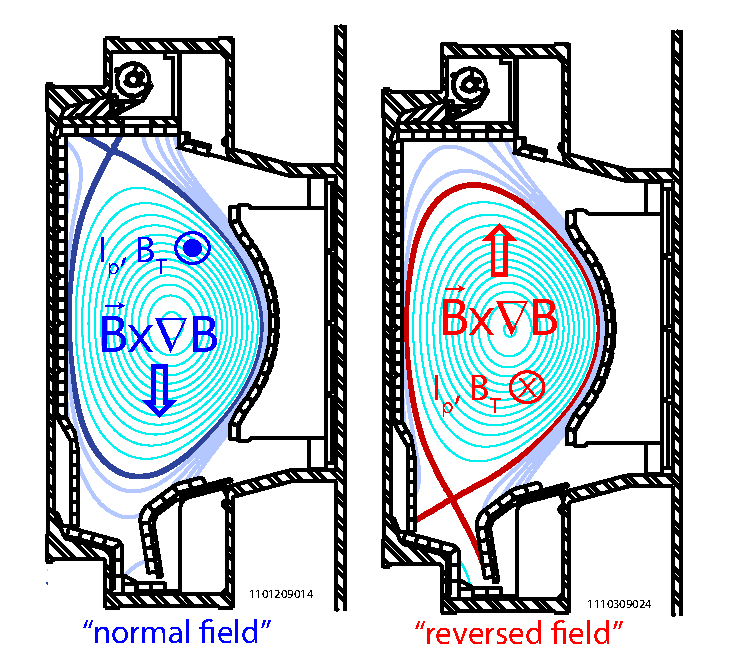
\includegraphics[width=100mm]{graphics/HighPerformanceRegimes/Shapes_USN_LSN.pdf}}
\end{figure}

I-mode access is fairly robust, provided the appropriate drift configuration is held -- this can be achieved either by running an upper-null shape, or by reversing the field (as well as the plasma current, to maintain magnetic-field helicity) and running in a standard LSN shape \cite{Hubbard2012}\gnote{graphic here}.  Upper-null operation allows a broader range of plasma shapes, but suffers from poorer diagnostic coverage and power handling due to the SOL flux impinging on a flat strike plate rather than the full lower divertor \cite{Hubbard2012,Dominguez2012}.  Short I-mode periods have also been observed in the favorable-drift configuration in a modified plasma shape used for ELMy H-mode experiments on C-Mod, but these transitioned quickly into H-mode and will not be considered for the balance of this thesis \cite{Dominguez2012,Hughes2013}\gnote{ref to description, prob chapter 4?}.  In either the forward-field USN or reversed-field LSN shape, I-mode access is favored by higher heating powers, low collisionality, and strong shaping \cite{Whyte2010}; as with all C-Mod operation, I-mode is accessible with purely RF heating, without external sources of momentum input \cite{Hubbard2012b}.  Unlike H-modes on C-Mod, I-mode operation is also largely insensitive to wall conditions due to the low impurity confinement \cite{Hubbard2012}.

Initially, access to I-mode was available within a relatively narrow window in density and heating power -- I-mode attempts with insufficient density were aborted by core radiation from high-$Z$ impurities generated by interactions between fast ions and the wall, while high-density or high-power cases tended to transition into an ELM-free H-mode \cite{Whyte2010}.  However, more recent experiments have greatly expanded both the available density and heating power range in I-mode, particularly by fueling into established I-modes to maintain sufficiently low density at the L-I transition \cite{Hubbard2012b}.  As of the most recent campaign, I-modes can be sustained for the current flat-top ($\sim 20\tau_E$) up to the maximum available RF heating power \cite{Hubbard2012,Hubbard2012b}.

\subsection{Global Performance \& Edge Behavior}\label{subsec:hcr_imode_performance}

I-mode is characterized by H-mode-like energy confinement ($H_{98} \sim 1$) while maintaining an L-mode density profile and particle transport level.  While the pedestal density is generally low, $n_{e,ped} \sim \SI{1e20}{\per\meter\cubed}$, pedestal temperatures are typically higher than H-modes at comparable power.  Due to profile stiffness in the core, this results in very high core temperatures, and global-average pressures near the C-Mod H-mode -- and therefore the all-tokamak -- record ($\sim\SI{1.5}{\atmosphere}$ in I-mode, compared to $\sim\SI{1.8}{\atmosphere}$ in H-mode) \cite{Hubbard2011}.  Notably, scalings of stored energy against RF power in I-mode indicate only weak degradation of energy confinement with heating power, contrary to the $\tau_E \sim P^{-0.5}$ (L-mode) or $\tau_E \sim P^{-0.69}$ (ELMy H-mode) scalings previously observed -- a potentially highly-favorable result for extrapolation to ITER-scale devices.  Particle and impurity confinement, on the other hand, is minimal, limiting 
radiative losses to $\sim 25\%$ of heating power, well below H-mode levels \cite{Whyte2010} -- impurity confinement times and accumulation are measured to be at L-mode levels on laser blow-off \cite{Howard2011} and charge-exchange \cite{McDermott2009,McDermott2009a} diagnostics.  Initial studies of the I-mode threshold indicate that the mode should be accessible on ITER at reduced density ($\sim \SI{4e19}{\per\meter\cubed}$), then fueled after the transition up to a $Q=10$ scenario \cite{Hubbard2012b,Greenwald2013}.  Ready fueling control in such a scenario would be critical, as density is the primary engineering ``knob'' for fusion power in predominantly self-heated fusion plasmas \cite{Hubbard2012}.

\begin{figure}
 \pushtooutside
 \ffigbox[\FBwidth]{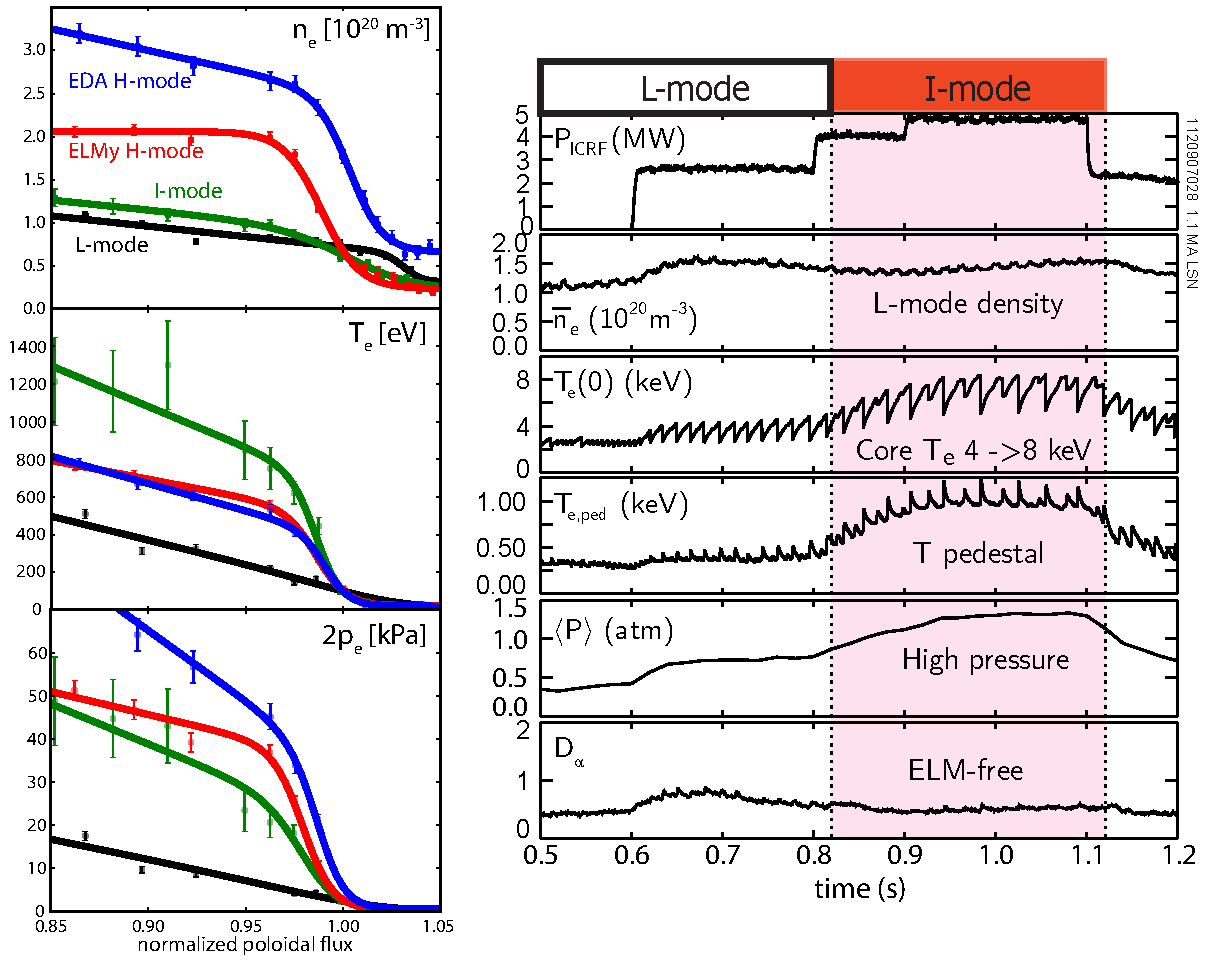
\includegraphics[width=150mm]{graphics/HighPerformanceRegimes/trace_imode.pdf}}{\caption[Characteristic traces for a typical I-mode, and comparisons of I-mode pedestal profiles to L- and H-modes.]{(right) Characteristic traces for a typical I-mode.  At the L-I transition, the core and edge temperature rise over several sawtooth cycles before reaching a steady level; global confinement and pressure rise accordingly.  However, the density remains at L-mode levels, and no ELMs are exhibited.  (left) Edge profiles for density, temperature, and pressure in L-, I-, and H-mode.  The I-mode (green) retains an density profile comparable to the L-mode (black), unlike the ELMy (red) and EDA (blue) H-modes which form a strong density pedestal.  However, the I-mode forms a taller temperature pedestal than either H-mode.  As a result, the I-mode reaches comparable pedestal pressures to the H-modes while retaining L-mode particle transport.}\label{fig:hcr_imode_trace}}
\end{figure}

\begin{figure}
 \pushtooutside
 \fcapside[55mm]{\caption[Impurity confinement time versus normalized confinement for L-, I-, and H-mode.]{Impurity confinement time $\tau_I$ measured by laser blow-off \cite{Howard2011} versus normalized confinement $H_{98}$ for L-mode, I-mode, and H-mode.  I-mode exhibits H-mode-like energy confinement, increased by roughly a factor of two over L-mode.  However, I-mode retains L-mode levels of particle and impurity transport, readily flushing heavy impurities from the plasma.  EDA H-mode exhibits strongly increased particle confinement, while transient ELM-free H-modes increase their particle confinement to the point of radiative collapse (see \cref{sec:hcr_elmfree})}\label{fig:hcr_imode_taui}}{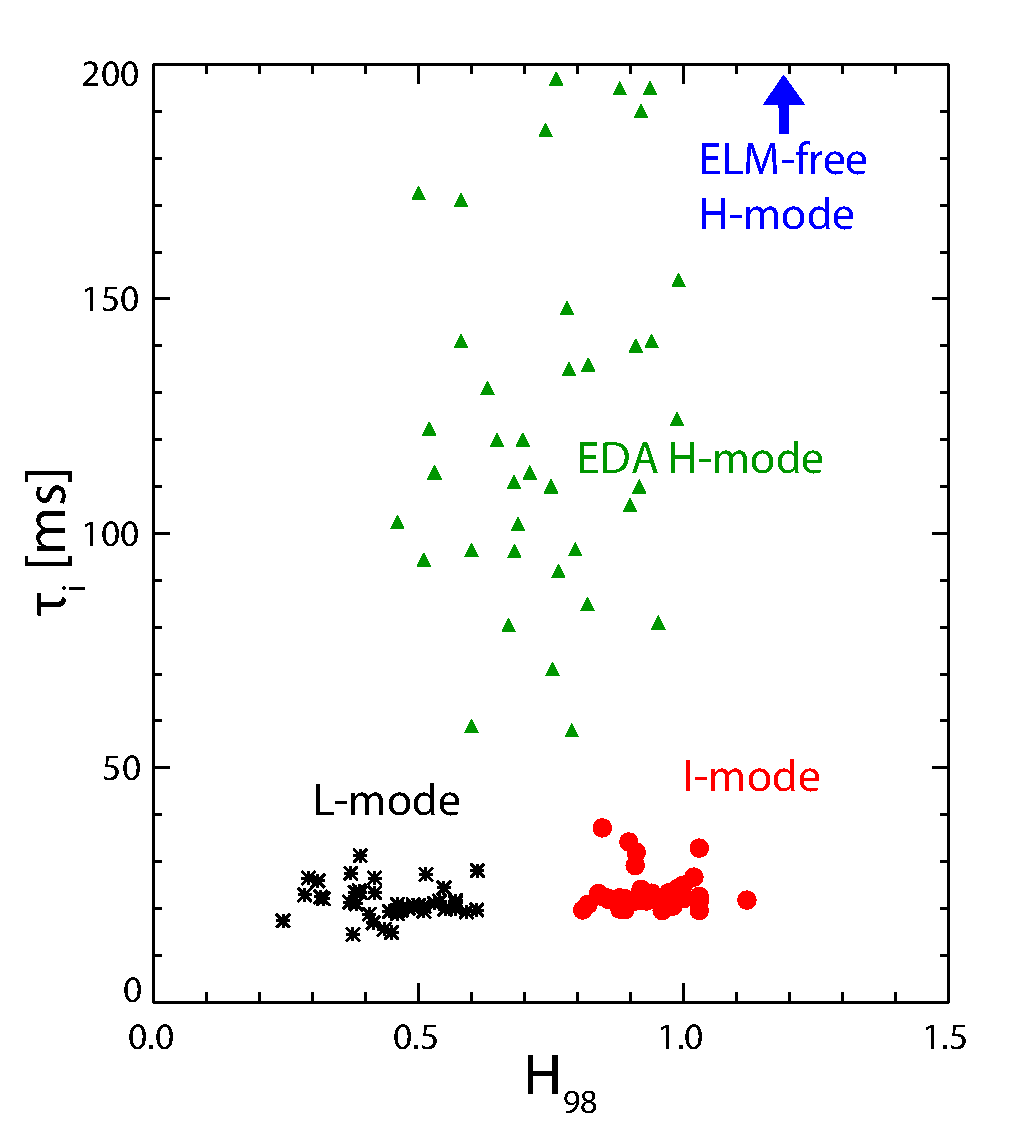
\includegraphics[width=90mm]{graphics/HighPerformanceRegimes/taui_h98.pdf}}
\end{figure}

The lack of a particle transport barrier in I-mode drives significantly different edge behavior compared to H-mode -- the reduced $\nabla n_e$ in the pedestal reduces both the overall pressure gradient and the bootstrap current drive\gnote{define bootstrap earlier?}, which has a stabilizing effect on both ballooning and kink/peeling edge MHD modes \cite{Hughes2013}.  The SOL heat flux channel in I-mode also appears to be significantly wider than in comparable H-modes \cite{Whyte2010,Hubbard2012b}.  Energy transport suppression in I-mode appears along with the expected $E_r$ well at the edge -- although historically I-mode $E_r$ wells are shallower and exhibit weaker shear than those in H-mode, more recent measurements have found comparable well depths in both regimes \cite{McDermott2009,Theiler2014}.  I-modes exhibit toroidal rotation levels comparable to H-mode, consistent with a $\nabla T_e$ scaling for rotation velocity \cite{Rice2011}, which may contribute to edge shearing in I-mode \cite{McDermott2009}.

Notably, the edge behavior across the L-I transition is distinct from more conventional L-H transitions.  While the L-H transition is a rapid ($\sim \SI{20}{\milli\second}$ on C-Mod) bifurcation in transport\gnote{reword, check values}, the L-I transition is marked by a slower, steady increase in edge temperature, lasting up to $\sim\SI{150}{\milli\second}$ \cite{McDermott2009,Whyte2010}.  The L-I transition appears to be tied to sawtooth heat pulses\gnote{explain sawteeth where?} reaching the edge -- with each heat pulse, the edge temperature ``ratchets'' upward, reaching a steady I-mode over several sawtooth cycles \cite{Hubbard2011,Hubbard2012}.  The L-I transition is seen to be more rapid at higher levels of RF heating power and lower $q_{95}$ \cite{Whyte2010}.  Both factors are associated with larger sawtooth crashes, consistent with a transient heat pulse driving the transition \cite{Hubbard2012}.

\subsection{Edge Fluctuations -- the Weakly-Coherent Mode}\label{subsec:hcr_imode_wcm}

\begin{figure}
 \pushtooutside
 \ffigbox[\FBwidth]{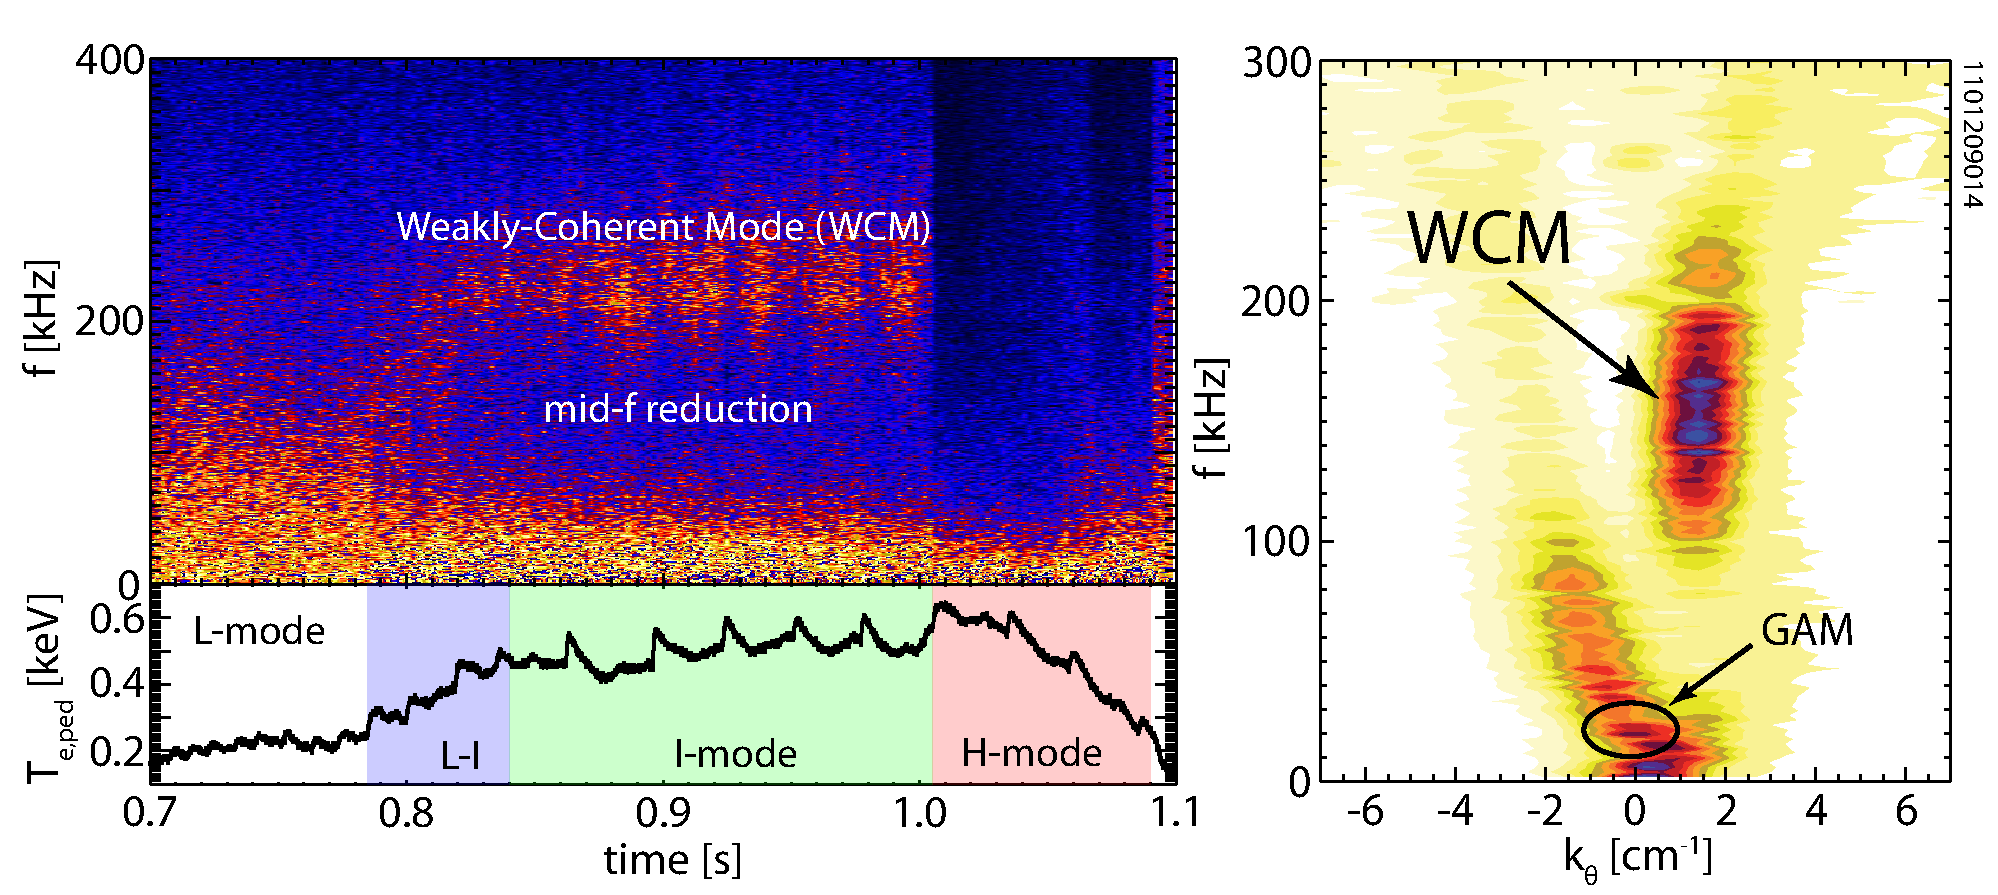
\includegraphics[width=150mm]{graphics/HighPerformanceRegimes/WCM.pdf}}{\caption[Fluctuations from the WCM in I-mode.]{Measurements of $\tilde{n}_e$ fluctuations from the WCM in I-mode.  (left) Reflectometer measurements in the pedestal region, showing the transition from broadband L-mode turbulence to the WCM, and subsequent fluctuation suppression as the plasma transitions into an ELM-free H-mode.  Edge $T_e$ measurements are also shown, tracking the formation of the characteristic I-mode temperature pedestal.  Note the dynamics of the L-I transition -- while the edge temperature increases steadily over several sawtooth periods, the turbulence suppression and formation of the WCM is more rapid, with the mode spinning up in frequency as the I-mode is established.  (right) Gas-puff imaging measurements of the WCM, averaged over the I-mode.  The mode is restricted in $k$-space to $k_\theta \sim \SI{2}{\per\centi\meter}$, but is broad in frequency.  Also shown is the $k_\theta = 0$, $f \sim 
\SI{10}{\kilo\hertz}$ signal of the 
GAM coupled to the WCM. \note{point to Cziegler here?}}\label{fig:hcr_wcm}}
\end{figure}

As with other high-performance regimes, the I-mode pedestal exhibits broadband suppression of turbulence at moderate frequencies ($20-150\;\si{\kilo\hertz}$).  In its place, the I-mode pedestal exhibits a broad electromagnetic fluctuation termed the \emph{Weakly-Coherent Mode} \cite{Whyte2010}.  The WCM is primarily observed as a density and magnetic fluctuation, although temperature fluctuations associated with the mode are also observed (albeit at an amplitude reduced by roughly an order of magnitude) \cite{Cziegler2013,Dominguez2012,White2011}.  Due to its prominence in the I-mode edge and similarity to the quasi-coherent mode (QCM) found in the EDA H-mode, the WCM is a prime candidate for pedestal regulation in I-mode, driving the enhanced density transport -- initial observations indicate a correlation between particle flux through the LCFS and the (normalized) WCM amplitude \cite{Dominguez2012}, although a firm characterization of the effect of the WCM on the particle transport is ongoing.

The WCM is found at fairly short poloidal wavelength, $k_\theta \sim \SI{1.5}{\per\centi\meter}$, similar to the QCM \cite{Dominguez2012}.  Compared to the QCM, however, the WCM is significantly less coherent -- $\delta f/f \sim 50\%$, compared to $\sim 10\%$ for the QCM -- and exists at a higher frequency ($200-400\;\si{\kilo\hertz}$) and phase velocity \cite{Hubbard2011,Cziegler2013}.  While the radial location and extent of the WCM has not yet been definitively determined, it has been localized within the last $\sim \SI{2}{\centi\meter}$ of the LCFS by O-mode reflectometry \cite{Dominguez2012} and gas-puff imaging \cite{Cziegler2011,Cziegler2013}.  The onset of the WCM is immediate and contemporaneous with the turbulence suppression in the L-I transition, unlike the formation of the $T_e$ pedestal, which typically requires several sawtooth cycles to form \cite{Cziegler2011}.  However, the WCM can ``dither'' for several sawtooth heat pulses in marginal I-modes, and typically spins up in frequency as the mode is established (contrary to the behavior observed in the QCM) \cite{Cziegler2011,Hubbard2011}.

The nature of the WCM is, as of this writing, an open question -- several candidate instabilities have been proposed, including a branch of the kinetic-ballooning mode \cite{Tang1980} or the heavy-particle mode \cite{Coppi2012,Coppi2012a}, but the underlying instability in the WCM remains unknown\gnote{elaborate on potential modes?}.  Notably, the WCM appears to be coupled to Geodesic Acoustic Modes (GAMs) in the plasma edge\gnote{general cite for GAM?}.  GAM dynamics have been associated with the L-H transition on other tokamaks, but GAMs are not seen in H-modes on C-Mod -- however, persistent GAMs co-existing with the mean flow in the edge are consistently seen in I-mode \cite{Cziegler2013}.  Interplay with GAMS appears to drive much of the physics of the WCM, but the nature of the relationship between the two is still the subject of active research.\nicechapterending

\bibliographystyle{../plainurl}
\bibliography{../references}